\documentclass[11pt]{article}
\usepackage{deauthor}
\usepackage{algorithmic}
\usepackage{algorithm}
\usepackage{xcolor}
\usepackage{xspace}
\usepackage{graphicx}
%\usepackage[caption=false]{subfig}
\usepackage{footnote}
\usepackage{hyperref}
\usepackage{multirow}
\usepackage{subfig}
\usepackage{enumitem}
\usepackage{comment}



\begin{document}

\title{Episodic Memory Integration of Personal Data in YourDigitalSelf}
\author{Varvara Kalokyri, Alexander Borgida, Amelie Marian\\
 Department of Computer Science, Rutgers University\\
v.kalokyri@cs.rutgers.edu, borgida@cs.rutgers.edu, amelie@cs.rutgers.edu}
\date{October 2023}

\maketitle

\begin{abstract}
Human episodic memory consists of past personal
experiences organized into episodes. It is a crucial
part of our lives, influencing our identity and interpersonal
relationships. A large variety of digital devices and apps capture personal digital traces (PDTs) of our daily experiences,  including
messages, time and/or location data, browsing and purchase history, etc. Our goal
is to reconstruct meaningful episodes from PDTs, in order to 
improve memory recall and aid individuals with memory problems. In addition to acquiring PDTs, this process faces many problems, including: 
the diversity and very large number of PDTs;
describing the episode types of interest; 
finding and  combining the relevant but very sparse set of PDTs that provide
partial evidence for a particular episode having occurred.


To address these challenges, the YourDigitalSelf project employs semantic modeling and integration techniques to associate  PDTs with events, themselves organized into prototypical narratives/plans called scripts. It introduces a formalized conceptual modeling language, hierarchical script definitions, and an evidence-based bottom-up approach to reconstruct script instances. A first evaluation of our implemented methodology using a mobile application demonstrates relatively successful integration of diverse digital traces and memory enhancement.  
 
\end{abstract}

\section{Introduction}
In today's world, digital devices are seamlessly integrated into our daily lives, transforming the way we engage with people and our surroundings. These devices generate and store various kinds of Personal Digital Traces (PDTs), such as e-mails and messaging, location data, calendar entries, check-ins, reviews, web searches, and purchase history.  These PDTs, serve as a partial record of individuals' lives, but  pose a challenge to users because the full collection is very large, highly heterogeneous, and distributed in space and time, making it difficult to access, search, and learn from.

Drawing inspiration from Vannevar Bush's visionary ``memex" concept, which can be seen as a personal data collection system, our work aims to exploit the potential of organizing personal data in order to aid remembering past events. By connecting the dots between personal information items, users can effectively retrieve specific memories or information in a coherent and meaningful way.

The goal is to discover evidence for users' actions from the digital traces these actions leave behind, and organize them into coherent episodes that look like  high-level complex and meaningful workflows, enhancing the user's ``autobiographical memory''. This could be especially beneficial for remembering routine experiences, which has been shown to be harder to recall  \cite{bradburn1987answering}. For example, users could use connections in their data to not only quickly retrieve digital artifacts, such as pictures from a trip, minutes from a meeting, or pictures from a birthday party, but also to retrieve specific information about events, such as the name of a restaurant they went to,  the title of a movie they watched, etc.

Our research takes a step forward in supporting human memory and recall through the concept of episodic narratives, rooted in psychology and cognitive science. It enables users to organize PDTs into cohesive episodes, creating a personal knowledge base that users can query to remember specific events and their by-products. Additionally, it provides users with narratives to stimulate their memory, which can be particularly helpful for those with memory difficulties.

To achieve this, we need to acquire and integrate all the  heterogeneous data from  various  sources, including files  used by apps on our devices (e.g., search history), and  through service APIs. We focus in this paper on the following aspects: 
\begin{enumerate}[noitemsep]
    \item  A conceptual model to represent entities, especially PDTs, which helps extract  semantically similar aspects (e.g., who? when? where?), thus {\em integrating}   the   heterogeneous sources.
    \item  A conceptual model for atomic activities/events. Note that PDTs may provide weighted evidence signaling the occurrence of an activity instance.
    \item A conceptual model of complex activities, called  {\em scripts}. These contain stereotypical commonsense plans, whose instances can again be signaled by the presence of either PDTs  or activities/sub-subscripts. A novel notion of inheritance and subsumption helps one to create and organize libraries of scripts.
    \item An   algorithm for  recognizing instances of atomic and composite events/scripts.  The bottom-up nature of the algorithm, which merges evidence for components, allows us to deal with missing parts or atypical instances of scripts;  a scoring scheme  accounts for the varied strength of evidence provided by PDTs or script steps.

%    \item A new merging algorithm to recognize instances of scripts from PDTs, resulting in a Personal Knowledge Base which utilizes
  %  \item A self-evaluating multiplayer web-based game for collecting digital trace descriptions for every step in a script scenario since apart from the script knowledge that we need for recognizing everyday activities, it is also necessary to collect enough explicit knowledge about the digital traces produced by each step of those scripts. 
  %   \item The design of YourDigitalSelf - a realization of our research methods through the development of a mobile application used as the basis to retrieve personal digital data originating from various sources and organize them into coherent episodes. 
  \item An Android app which instantiates our ideas, asking users to
provide access to a specific set of data sources, loading the data
into the PDT concepts, and running the above algorithm. 
  This application is also used to evaluate our approach, through user studies and surveys.
\end{enumerate}
 
We immediately acknowledge the sensitive nature of the personal data we are dealing with, and the very important privacy issues that they raise. All information  obtained to evaluate our work resides on individuals' own mobile phones without disclosing any personal information.

Our study results demonstrate the potential of our approach, showing its effectiveness in integrating digital traces from different sources into coherent episodes and enhancing users' memory of past actions. Our ultimate goal is to empower users to create their personal knowledge base and better manage their digital memories.


\section{An episodic script model for personal digital traces}

Our approach to data integration and memory recall draws on principles from Cognitive Science and Psychology, specifically in the study of how individuals reminisce about their past experiences. These psychological findings have yielded several key observations.

The Natural Mnemonic Framework: It is observed that when people reflect on their past, they often do so by responding to a set of fundamental questions, which we refer to as the `w5h' questions: what, when, where, who, why, and how \cite{schacter, jones}. For instance, when attempting to recollect a significant event like one's sixth birthday, individuals instinctively seek to reply to these contextual cues. We use this inherent cognitive framework as the foundation of our data integration,  by aligning PTDs and conceptual model instances along these essential questions.

Episodic and Semantic Memory: Psychological research \cite{tulving, conway} distinguishes between two primary forms of memory. Semantic memory pertains to the accumulation of general world or cultural knowledge that individuals collect over their lifetimes (e.g., it encompasses the understanding that payment is required when making a purchase) and episodic memory involves the capacity to re-live specific past events or episodes, (such as the memory of celebrating one's 40th birthday by dining out).  Our approach  combines the representation of both semantic memory (scripts) and episodic memory (script instances). This fusion allows us to assist users in recalling information related to past events. To achieve this, it is imperative to connect individual atomic events and organize them into broader activities, even when these events occurred at different times. This linkage facilitates the retrieval of high-level activity-based memories, enhancing the user's ability to reconstruct their personal history effectively.

\subsection{Conceptual modeling of personal digital traces}
As mentioned, our objective is to develop a framework for modeling digital traces that unifies information based on the `w5h' questions. To achieve this, we start with a standard-centered conceptual modeling language, as first presented in \cite{usOdbase}. This language employs entity classes, such as `Documents' and `Persons,' which contain individual instances. These instances possess atomic valued {\em features}, such as the size of a document, and are interconnected through {\em properties}, such as those associated with an Email, including `from,' `to,' `date', `subject,' and `body.'

Within this modeling framework, classes can be specialized  into subclasses. For instance, `PERSON\_WITH\_EMAIL' is a specialization of the `PERSON' class, and new properties, such as `email\_address', can be introduced, or existing properties may be further constrained.%, as in the case of setting age restrictions ($>$13). 
Notably, properties can also undergo specialization, where, for example, `from' and `to' are sub-properties of `who'. A large subset of the properties of PDTs can be viewed as specializations of w5h, when these are viewed as properties themselves, resulting in the integration of heterogeneous object schemas. 

Note however that there is no sensible way to ask questions like ``when?" or ``who?" of many objects.  However, by associating an object with a primitive action, it becomes possible to derive the `when' aspect from the action. For instance, we may not directly ask `who email', but we can ascertain `who sent an email'. This requires attaching documents to primitive actions.%, followed by the grouping of these actions into more complex events resulting in coherent episodes.

\subsection{Conceptual modeling of atomic and complex events}

A script-based model is adopted for the purpose organizing atomic actions into coherent episodes. This describes event flows, encompassing steps that humans intuitively understand. For example, for going out to eat, these include steps like organizing the outing, making reservations, taking transportation, and making payment. These steps often generate PDTs, serving as evidence for the activities. 
For example, we then want to group emails concerning a particular dinner, a reservation that was made at a restaurant, a Facebook check-in with photos, and a credit card payment. The atomic actions  that generated these documents are organized
 as part of the narrative for going out to eat.  Essentially, each data trace presents evidence of various strengths for the occurrence of atomic event instances.

To achieve this, we need a set of higher-level plans that the users and their community frequently engage in, which describe the connections between all those events. The idea of scripts is inspired by the work of Schank and Abelson in AI\cite{schank1977}, which are defined as plans describing stereotyped sequences of actions that describe some well-known situation.

For describing such scripts we use the standard notation used in business process management (BPM)\cite{declarativeBPM15}. As such, scripts are characterized by their goals, participant information, w5h aspects, component sub-scripts, and allowed sequencing and timing of sub-scripts/atomic actions - the latter captured in BPM. 

However, in order to make a fully functional system, we need script definitions for many variants of everyday activities. These plan descriptions serve as prototypes due to the vast variability inherent in such situations, making it impractical to predetermine every possible variation. This will be facilitated by placing the script definitions in an ontology and then using specialization and inheritance, so that more specific processes, such as GoingOutToEat, GoingOutToConcert, GoingToOpera, etc. are obtained by indicating only differences from a common superclass, GoingOutForEntertainment. In turn, GoingOutToEat can be specialized to EatingOutAtRestaurant, EatingFastFood, etc. By using specialization hierarchies we can organize large knowledge bases, support reuse and change propagation, as well as prevent repetition errors.

Description logics (DLs) are ideal for the creation of specialization of such hierarchies via reasoning.  We have introduced a new extended regular expression-based Description Logic \cite{borgidaai4bpm} able to represent the control flow semantics of structured BPM .%and therefore represent our scripts and be able to reason about them. 
For example, specific concepts A and B can be specified, and then we can assert that a class A is subsumed by B, or discover this relationship by reasoning, meaning that all instances of A are instances of B. We can also detect inconsistencies, (e.g. we might give a description of going out to a rock concert which contradicts going out to a concert. This will provide evidence that this is not a proper specialization).

Instance recognition for DLs by the use of inference could be used for our purposes for recognizing activities. However, this approach cannot be used because: not all steps occur in every instance, their order may vary, and some steps may leave no digital trace. Instead, a bottom-up approach is proposed where partially instantiated scripts are constructed from individual PDTs, and compatible instances are merged, accumulating information and strengthening evidence for them. This approach is flexible and accommodates various types of scripts, making it suitable for different scenarios. In the next section, the algorithm for creating episodes from PDTs is described.

\section{Algorithm for Episode Recognition}
Our algorithm, starts with a specific script (S) and a comprehensive set of PDTs (P). The primary objective is to generate potential script episodes, which are instances of (S), and establish connections with the PDTs.

\textbf{Step 1. Script Specification:}
A script specification has the following components: a top-level (outer) script (e.g. `EatingOut' script), which we want
to instantiate; several component sub-scripts and atomic actions; as well as sequencing relationships among them. In addition, every script  contains its w5h properties. 

For example, `EatingOut' comprises  events like inviting people, making reservations, going to a restaurant, paying the bill, and sharing photos. Some of these events (e.g., making a payment) offer strong evidence that the person indeed participated in this activity/script. On the other hand, receiving an email mentioning ``dinner" or ``lunch" provides weaker evidence for planning to dine out, which, in turn, offers weaker evidence of actually going out since the plan may remain incomplete or canceled. Our algorithm employs the concept of strong and weak evidence to prioritize potential script instances.

We gather information about the strength of evidence in a similar manner to acquiring common-sense knowledge about events within a given context. For that purpose, we have developed a self-evaluating multiplayer web-based game for collecting digital trace descriptions for every step in a scripted scenario and potential strength of evidence \cite{kalokyri2023one}. It is essential to note that there are limited ``objective" methods for scoring evidence because scripts represent imprecise, culturally-shared, commonsense knowledge describing typical human activities.

\textbf{Step 2. Retrieving Document Set for Script Instantiation:}
Once a script is parsed, the subsequent task involves identifying the set of documents, denoted as (D), that serve as evidence for the occurrence of its instances. These documents correspond to PDTs and act as ``noisy sensors," indicating potential instances of corresponding scripts or atomic actions for which strong evidence exists.

To locate documents that correspond to a specific piece of evidence, it is crucial to identify specific cues within the documents. These cues can take the form of verbs to search for (e.g., ``eat" in an email to identify an ``Initiate Going Out" event) or attributes and metadata that a document may possess (e.g., categorizing a payment as ``Restaurant" or ``Supermarket" to find evidence for ``Making a Payment at a restaurant or supermarket respectively). To ensure the replicability of this process for various scripts, the w5h components of the script or atomic action are obtained from its FrameNet frames\cite{fillmore2003background}. Standard sources of synonyms and hyponyms such as WordNet and ConceptNet5 \cite{miller1995wordnet, liu2004conceptnet} are then utilized to identify additional words for searching. The generated lists of words and phrases from this process are stored in a text file and used to retrieve all potentially relevant documents.

Finally, the set of documents (D) is pre-processed by: (i) expanding information (e.g., terms like ``tomorrow'', ``on Friday'', are made absolute dates); (ii) performing entity resolution for people and places (who and where dimension) using Stanford's Entity Resolution Framework \cite{serf}; (iii) grouping certain kinds of documents (e.g., related email threads, or related sequences of tweets) into a single individuals d in (D); (iv) finding the places/venues that the user has visited from the geo-location coordinate history (gps) \cite{li2008mining}. 

\textbf{Step 3. Creating Initial Script Instances:}
Every document in the set (D) serves to instantiate atomic actions or sub-scripts, creating candidate instances of the outer script (S) in a bottom-up fashion. Similarly, the w5h properties are propagated from the document into the atomic actions and the script hierarchy.

\textbf{Step 4. Merging Script Instances:}
Merging script instances is a distinctive feature of our system, using multiple sources of evidence for the same script instance. Each script is assigned ``keys" that rate the importance of w5h (sub)properties in identifying instances. For `EatingOut', the keys are `whereEatingOccurred', `whenEatingOccurred', and, to a lesser
extent, `who'. The `what' and `how' properties of this script are not important because they would often lead to incorrect merging (e.g., two instances of eating pasta (`what') need not be merged). Since
every script can have different keys, this has to be explicitly mentioned in the algorithm. When two instances share similar keys, they are considered candidates for merging. The w5h property fillers are combined, and a score is computed for the merged instance based on Hooper's rule \cite{shafer1986combination} for combining probabilistic evidence.

The key point here is that the merging process cannot be completed in a single step. After the script instance is established with a certain degree of certainty, additional PDTs may be collected as part of the instance when examining the script definition.

\section{A mobile app for YourDigitalSelf}
%: A Personal Digital Trace Integration Tool}

So far, we have given in Section 2 an ontology of entities (especially for
PDTs), and of atomic and composite events/scripts, which
involve these entities. In Section 3, we discussed how specific PDT concepts
provide evidence of varying strength for specific scripts,
and an algorithm which, given a script (episode type), uses this information to
instantiate very small episode fragments and then merge them into
larger ones, with associated strengths.

To build our YourDigitalSelf Android app (see
\cite{kalokyri2018yourdigitalself} for details, including screen shots), we first
need to have {\em users} provide access to the data sources from
which the PDT instances will be created, and then interactively choose
a specific script for which they wish to see rank-ordered instances
retrieved. 
The types of PDTs along with the data sources currently supported by the app are the following:
 \begin{itemize}[noitemsep, topsep=1pt]
     \item {Messaging: Messenger, phone text messages}
     \item {Social Media: Facebook, Instagram}
     \item {Email: Gmail}
     \item {Calendar: Google Calendar}
     \item {Financial Data: Plaid API and directly downloaded .csv files from bank institutions}
     \item {Location Data: Google Maps location history, GPS data}
     \item {Photos: Google Photos}
 \end{itemize}
The system then gathers the raw data and uses it to populate the
corresponding PDT concepts.  In
general, each API has a standard format, but in the
not-infrequent case where APIs change, this mapping must be modified.
Recall from Section 2.1 that properties for the 'w5h' questions and their
sub-properties are the key to semantically ``integrating'' the extremely heterogeneous forms of PDTs.

%??   possibly forcing the use screen scraping.

When asked, the app then essentially runs the algorithm in Section 3 to
 gather episodes (script instances) of the script asked for, and then
 displays them via a GUI. Note that each episode has attached a variety of PDTs that provided evidence for it; this is a second way in which related data is ``integrated''.

Instances of the concepts in  conceptual model  cannot be efficiently
 stored directly on the mobile phone, and must instead be mapped to a
relational database natively managed by Android. The mapping of the
different concept types to tables is declaratively described using
pairs of conjunctive queries.

%Should we have this paragraph
After the mapping to our model, the next step involves
designing an indexing structure to facilitate data queries. We
leverage a combination of full-text and column indexing techniques
provided by the Android platform. The indexing occurs whenever the
user decides to include data in the app, either manually or through
automated periodic updates.


In general, the project has made a significant effort to support
extensibility and modification by {\em declarative} representation
of other aspects as well, such as evidence to look for in scripts and clues to
search in PDTs, as well as making scripts parametric/generic (e.g,
Book$<$T$>$, T=``accommodation", ``concert",...).


\subsection{Experimental Setup}

To assess the effectiveness of our approach, we conducted experiments using real user data with the primary objective of detecting instances where individuals engaged in dining out at restaurants. We opted for this specific script example because it offers a rich variety of PDTs and shares commonalities with other scripts related to entertainment, such as attending theaters or concerts. 

We employed the YourDigitalSelf Android application for this purpose, which allows users to install it locally on their devices, and it is designed to serve future research purposes as well. It is paramount to clarify that our approach did not entail direct access to users' personal data. Instead, users provided responses solely in the form of Yes/No answers, without revealing any personal information. The application is configured to collect PDTs from a diverse range of services, including messaging, social media, email, calendar, financial data, location data, and photos.

We ran an in-depth study\footnote{Our study has received approval from the Rutgers University Institutional Review Board (IRB) committee.}  with 16 users. Before the experiment, we asked participants to try to remember the occasions of them going out to eat at restaurants and then carefully go over their past month's digital information, writing down their outings, including name of the restaurant - where, date they went - when,
with whom they went - who. We used this information as a proxy for recall.
Then during the experiment participants were shown all candidate script instances of them going out to eat at restaurants, and had to indicate Yes/No for each of the instances first, and then for each of the w5h properties.

For a comprehensive description of the entire study and its results, we refer interested readers to the detailed study in \cite{kalokyri2022supporting}. 

%In total, we received responses from 42 participants. These responses shed light on the diverse sources that users employ for each of the five primary sub-scripts related to dining out. Notably, users exhibited a wide range of behaviors. The majority relied on traditional communication methods, such as plain text messages or phone calls, for coordinating restaurant outings. In contrast, some users preferred digital messaging applications, emails, and a smaller portion made use of platforms such as Snapchat, Whatsapp, and Groupme. On another note, users demonstrated a degree of unanimity when it came to making restaurant reservations (predominantly via phone) and the type of payment (credit card or cash). Furthermore, it was observed that users did not consistently maintain digital records of their restaurant outings. Additionally, users employed diverse sources to inform their friends about their restaurant visits, with Instagram and Facebook being the predominant choices. Interestingly, 31\% of users reported not using any online service for this purpose.

%These findings underscore the significance of considering multiple sources of PDTs when seeking to identify script instances for individual users. Any approach aimed at retrieving user memories must exhibit adaptability to accommodate the broad spectrum of user behaviors.

\subsection{Experimental Evaluation}
 The evaluation of our approach focuses on the assessment of our matching algorithm and scoring function which encompasses two key aspects: (1) the effectiveness of our approach in identifying script instances and (2) its proficiency in recognizing and abstracting `When,' `Where,' and `Who' information from sub-scripts and atomic actions into the overarching script instance.

For both facets of evaluation, we employ two distinct dimensions of relevance:
\begin{enumerate}[noitemsep]
    \item \textbf{Binary Relevance}\\
    A script instance is deemed relevant if the user actually engaged in dining out at a restaurant, even if the `w5h' information was only partially correct whereas each `w5h' information is considered relevant only if it is precisely correct (neither a subset nor a superset). 
\item \textbf{Graded Relevance}\\
A proposed script instance falls into one of the following categories:\\
Exactly relevant: When the user indeed dined out at the specified restaurant.\\
Relevant but too broad: When the identification of a restaurant outing is accurate, but the user's purpose for the visit did not involve dining (e.g., for dancing or socializing with a friend).\\
Relevant but too narrow: When a restaurant outing is correctly identified, but the user did not stay at the establishment to eat (e.g., it was a takeout order).\\
Partially relevant: When a planned outing was correctly identified, but the user did not follow through with it.\\
Not relevant: When the identified instance does not pertain to a restaurant outing.

We establish an analogous framework for assessing the relevance of `When,' `Where,' and `Who' (`w5h') information, classifying them into relevant categories based on the same criteria.    
\end{enumerate}

To measure the performance of our approach, we rely on the following metrics, considering both binary and graded relevance:
\begin{itemize}[noitemsep]
    \item \textbf{Percentage of instances retrieved:} This metric indicates the percentage of all `EatingOut' events identified by users that our scripts successfully retrieved. It serves as a proxy for recall.
    \item \textbf{Mean Average Precision @ k (MAP@k):} Utilizing MAP as a binary relevance assessment, we determine the percentage of the top-k identified script instances that correspond to actual `EatingOut' events. 
    \item \textbf{Normalized discounted cumulative gain (nDCG):} This metric is employed to assess the ranked results while considering graded relevance, as described earlier. 
\end{itemize}

\subsection{Experimental Results}

Table~\ref{table:events-retrieved} shows the number of correct EatingOut instances retrieved by our approach compared with the number identified by users from memory, and by searching their PDTs. A first observation is that the results clearly indicate how hard is for users to recall their outings, either from memory or even when asked to go through their digital information. 
Our approach identified more correct instances than the users were able to recall and find in all cases but two (users 3 and 9 in bold). In addition, users found it hard to search through their data, since most of the applications have keyword-based search. Users 5 and 6 in bold, who were able to retrieve only half of their outings, clearly show this issue. 

\begin{table*}
\scriptsize
\begin{center}
{
\begin{tabular}{|l||c|c|c|c|c|c|c|c|c|c|c|c|c|c|c|c|}
\hline
  & \#1 & \#2 & \#3 & \#4 & \#5 & \#6 & \#7 & \#8 & \#9 & \#10 & \#11 & \#12 & \#13 & \#14 & \#15 & \#16\\
\hline
\hline
Our approach  & 13 & 15 & 10 & 5 & \textbf{14} & \textbf{24} & 13 & 6 & 19 & 17 & 19 & 7  & 11 & 5 & 17 & 15\\
\hline
User memory  & 7  & 8  &  8 & 5 & 8 & 10 & 5 & 5 & 9 & 9 & 13 & 5 & 6 & 3  & 8 & 9\\
\hline
User data  & 13  & 14  &  11 & 5 & \textbf{7} & \textbf{14} & 11 & 6 & 20 & 14 & 15 & 5 & 11 & 5  & 16 & 14\\
\hline
\hline
\textbf{Recall}  & 1 & 1 & \textbf{0.91} & 1 & 1 & 1 & 1 & 1 & \textbf{0.95} & 1 & 1 & 1  & 1 & 1 & 1 & 1\\
\hline
\end{tabular}
}
\caption{Number of identified EatingOut actions by users vs number of correct events our approach retrieved per user as a proxy for Recall}
\label{table:events-retrieved}
\end{center}
\end{table*}


\begin{table*}
\scriptsize
\begin{center}
{
\begin{tabular}{|l||c|c|c|c|c|c|c|c|c|c|c|c|c|c|c|c|c|}
\hline
  & Sources &  \textbf{Precision}\\
\hline
\hline
User \#1 & Social Media, Calendar, Financial Data, Location Data, Google Photos & 0.87 \\
User \#2 & Social Media, Location Data, Financial Data &\textbf{0.94} \\
User \#3 & Email/Messaging, Social Media, Calendar, Financial Data & 0.66\\
User \#4 & Email/Messaging, Social Media, Calendar, Financial Data, Location Data, Google Photos & 0.66 \\
User \#5 & Email/Messaging, Social Media, Calendar, Financial Data, Location Data & 0.74\\
User \#6 & Social Media, Calendar, Financial Data, Location Data, Google Photos & 0.89 \\
User \#7 & Email/Messaging, Social Media, Calendar, Financial Data, Location Data, Google Photos & 0.76\\
User \#8 & Email/Messaging, Social Media, Calendar &\textbf{0.6} \\
User \#9 & Email/Messaging, Social Media, Calendar, Financial Data, Google Photos & 0.74 \\
User \#10 & Email/Messaging, Social Media, Calendar, Financial Data, Location Data & 0.81\\
User \#11 & Email/Messaging, Social Media, Calendar, Financial Data, Location Data, Google Photos & 0.76\\
User \#12 & Social Media, Calendar, Financial Data, Location Data, Google Photos & 0.86\\
User \#13 & Email/Messaging, Social Media, Calendar, Financial Data, Google Photos & 0.73\\
User \#14 & Email/Messaging, Social Media, Calendar, Financial Data, Location Data, Google Photos&  0.83\\
User \#15 & Email/Messaging, Social Media, Calendar, Financial Data, Google Photos & 0.77\\
User \#16 & Email/Messaging, Social Media, Calendar, Financial Data, Location Data, Google Photos & 0.79\\
\hline
\textbf{Total} & &\textbf{0.78}\\
\hline
\end{tabular}
}
\caption{Overall precision for each user}
\label{table:precision}
\end{center}
\end{table*}

Table~\ref{table:precision} shows the overall precision of the identified script instances along with the sources each user incorporated in the application. Our approach achieves a total precision of  78\% for all the users. User\#2 achieved the highest precision of all, since the sources they chose to include in the study contained bank transactions, google maps location history, Instagram and Facebook, sources that tend to be of high quality, whereas User\#8 achieves the lowest precision of all since they included their private phone text messages without any high-quality source. 

However, retrieval systems typically return results in a ranked order, and users expect the first few results to be the most relevant.  We now look at the quality of the returned answers by evaluating the mean average Precision@k metric. 

Figure~\ref{fig-MAP} shows the Mean Average Precision@k for all the identified script instances for all the users. As shown, our approach achieves a really good precision even for low values of k. The reason for that is that our approach does include many different kinds of sources and is able to account for all the different kinds of user behavior. 

Figure~\ref{fig-nDCG} shows the normalized discounted cumulative gain (nDCG) for the ranked results when taking into consideration the graded relevance. The nDCG was computed by normalizing the DCG@k with the ideal DCG value or IDCG@k. It is clear that our ranking quality is high, and our approach is able to recognize and distinguish highly relevant PDTs in favor of irrelevant PDTs.
\begin{figure*}[!htb]
\centering
\begin{minipage}{.48\textwidth}
  \centering
  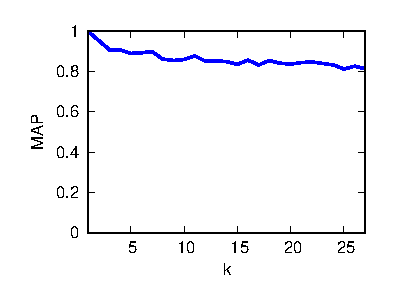
\includegraphics{submissions/Marian2023/plots/MAP.eps}
  \captionof{figure}{MAP@k for the recognized instances}
  \label{fig-MAP}
\end{minipage}\hfill
\begin{minipage}{.48\textwidth}
  \centering
  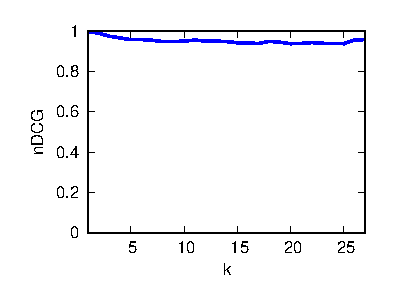
\includegraphics{submissions/Marian2023/plots/nDCG.eps}
  \captionof{figure}{nDCG@k  for the recognized instances}
  \label{fig-nDCG}
\end{minipage}\hfill
\end{figure*}

\begin{figure*}[!htb]
\begin{minipage}{0.48\textwidth}
  \centering
  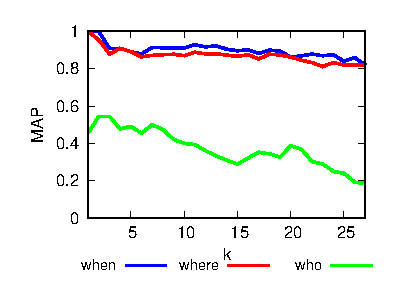
\includegraphics{submissions/Marian2023/plots/w5hMAP.eps}
  \captionof{figure}{MAP@k for when, where, who dimensions}
  \label{fig-w5hMAP}
\end{minipage}\hfill
\begin{minipage}{0.48\textwidth}
  \centering
  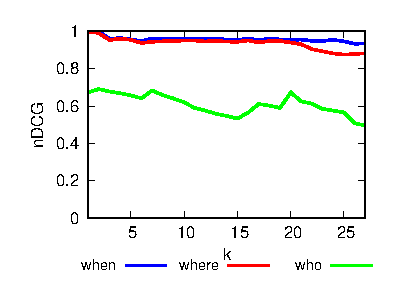
\includegraphics{submissions/Marian2023/plots/w5h_nDCG.eps}
  \captionof{figure}{nDCG@k for when, where, who dimensions}
  \label{fig-w5h_nDCG}
\end{minipage}\hfill
\end{figure*}


\begin{table}
\begin{center}
{
\begin{tabular}{|l||c|c|c|}
\hline
 & when & where & who \\
\hline
\hline
MAP& 0.85 & 0.81 & 0.21 \\
\hline
\end{tabular}
}
\caption{MAP for when, where, who dimensions for all users}
\label{table:w5h_MAP}
\end{center}
\end{table} 

We then report the same metrics (MAP, MAP@k, and nDCG@k) on the when, where, and who dimensions.
Table~\ref{table:w5h_MAP} shows the MAP for the three dimensions for all users. We observe that the when and where dimensions are easier to extract than the who dimension due to the metadata that the PDTs have. On the other hand, the who dimension is more difficult to extract. For example, we observe in figure~\ref{fig-w5hMAP} how the precision for the who dimension drops significantly as k increases. This happens due to the fact that for low values of k, the score of the instances is low, which means there are not many digital traces to account for these instances, therefore either there is no information, or our approach either lacks or recognizes more people in an outing. This is actually demonstrated in figure~\ref{fig-w5h_nDCG}, which shows the normalized discounted cumulative gain for the ranked results where we can now observe how much better the accuracy is for the `who' dimension. 

\section{Literature Review}
In this section, we provide a brief overview of various related research areas, highlighting the interdisciplinary nature of our work.

\textbf{Personal Information Management:}
Personal Information Management (PIM) research, dating back to the 1980s, focuses on assisting users in managing and organizing digital data. Researchers have suggested PIM interfaces for web activities \cite{stuff,kaptelinin2003umea,murakami2012system}, email \cite{ayodele2012machine,whittaker2006email}, and local files \cite{barreau1995finding,barreau1995context}. Existing systems often utilize domain-specific ontologies to identify relevant objects and their relationships \cite{haystack,ontopim}. In contrast, our approach is dynamic, emphasizing the integration of PDTs through narrative connections, shifting the focus from static information to dynamic data integration based on the `who, what, when, where, why, and how' (w5h) properties. 

\textbf{Process Representations:}
Our interest lies in representing autobiographic events and their instances. This area intersects with various formal process representation languages, graphical notations, and complex event recognition \cite{yawl2005},\cite{declarativeBPM15}. While traditional formalisms concentrate on enacting processes, we focus on descriptive formalisms that enable script instance recognition, underlining the challenges of recognizing multiple, concurrent, and personalized script instances. This leads us to
several relatively closely related areas such as Activities of Daily Living, Ambient Intelligence, Pervasive Computing, and LifeLogging. The following are some papers that survey an entire field
(e.g. LifeLogging  \cite{lifelogging}) or the use of ontologies and inference
\cite{bikakis2007survey,behavRecognitionSurvey14,alevizos2017probabilistic}.

\textbf{Activities of Daily Living, Pervasive Computing, LifeLogging, and Memory Tools:}
Memory aids play a crucial role in rehabilitation, particularly in improving prospective memory. Existing tools like Sensecam  \cite{hodges2006sensecam}, and Kalnikaite's browser \cite{kalnikaite2010now}  are akin to our approach, as they aim to trigger autobiographical memory by recording images and linking them to daily activities. Other tools include the MemoClip , the Cyberminder, and Memory Glasses \cite{memoclip,devaulmemory,deycybreminder}. However, we stand out by using pre-existing digital traces rather than capturing new data. In addition, the area of life-logging is quite similar, and is
surveyed in \cite{gurrin2014lifelogging,van2012introduction}. Bell has pioneered this field with MyLifeBits \cite{mylifebits} for which he digitally captured all aspects of his life. A recent paper \cite{timelinebuilder} focuses on the creation of lifelogs, positioning them as a critical resource for personal assistants to provide tailored advice within specific contexts. Another relevant paper is that of Meditskos et al \cite{meditskos2018multi} which used the technique of multi-sensory data analysis along with egocentric video recording from a bracelet to aid the dementia patients recognize their daily living activities.

\textbf{Planning:}
Plan recognition, a prominent field in AI, focuses on recognizing plans from actions \cite{planDagstuhl11,BuiBook}. Some similarities exist with our approach, particularly in recognizing multiple, concurrent, and interleaved script instances. We emphasize data integration, while traditional planning approaches are concerned with action sequences and transitions.

\textbf{Personal Digital Assistants:}
Personal Digital Assistant (PDA) systems, exemplified by Amazon Alexa, Siri, and Google Now, share commonalities with our work. These systems are engineered to provide users with event reminders based on their personal data, often driven by commercial objectives. However, their functionality is confined to utilizing data within the vendors' proprietary ecosystems. It's noteworthy that these PDA systems primarily emphasize future tasks, offering reminders based on time or event triggers \cite{schacter2002seven}. In contrast, our current application scenarios center around retrospective tasks, particularly the organization of past memories. Nonetheless, our data integration approach can complement prospective methods for tailoring activity recognition. 

Our approach emphasizes the dynamic integration of Personal Digital Traces (PDTs) through narrative connections and the recognition of multiple, concurrent, and personalized script instances, setting it apart from conventional methods in these related areas.


\section{Conclusion}
In summary, our research takes steps forward in advancing autobiographical memory by linking diverse PDTs based on their shared objectives, organizing them into cohesive episodic narratives. We introduced a conceptual model encompassing entities, PDTs, and the actions that create them. Scripts, which describe complex activities and are amenable to reasoning via description logic, played a pivotal role. Our merging algorithm identifies script instances, providing a valuable resource for users.
Through the YourDigitalSelf app, we evaluated and underscored the potential and promise of our approach. 

However, several directions for future research and development are worth considering. These include conducting a more extensive array of experiments encompassing a variety of scripts and involving a larger, more diverse population. Additionally, we recognize the necessity of incorporating Natural Language Processing (NLP) analysis to address instances where users mention activities indirectly. This could be potentially tackled with the use of today's natural language capabilities (such as openAI's chatGPT).
Beyond its implications for personal data management and memory enhancement, our work offers  opportunities for behavioral researchers. The combination of personal digital traces, AI, and self-reported surveys holds the potential to yield fresh insights into mental health assessment. 
Our tools are open source and publicly accessible on GitHub. This availability paves the way for educators and students to engage with their personal databases, fostering the development of novel, useful applications. Finally, our tools hold potential significance in the medical field, particularly for medical experts conducting studies related to memory rehabilitation in patients facing cognitive difficulties.

\bibliographystyle{ieeetr} 
\bibliography{submissions/Marian2023/references}
\end{document}
